\chapter{कृत्रिम बुद्धिमत्ता का परिचय}
\label{ch:intro}

\lakshyaheading
\begin{itemize}[leftmargin=1.4em]
  \item कृत्रिम बुद्धिमत्ता (Artificial Intelligence) का अर्थ एवं विज्ञान में इसका महत्व।
  \item AI, Machine Learning (ML) एवं Data के बीच सम्बन्ध।
  \item विज्ञान के प्रयोगों में AI किस प्रकार सहायक होती है।
  \item बिना कोडिंग के AI का अनुभव करने वाली सरल गतिविधियाँ।
\end{itemize}

\section{कृत्रिम बुद्धिमत्ता क्या है?}

जब कोई मशीन (machine) ऐसा कार्य करती है जिसके लिए सामान्यतः मानव-बुद्धि की आवश्यकता
होती है - जैसे देखना, पहचानना, भाषा समझना, या निर्णय लेना - तो उसे
\term{कृत्रिम बुद्धिमत्ता}{Artificial Intelligence, AI} कहते हैं।

उदाहरण के लिए, जब आपका मोबाइल आपके चेहरे को पहचानकर अनलॉक होता है, या जब Google आपकी
बोली हुई बात को टेक्स्ट में बदल देता है, तब पर्दे के पीछे AI ही कार्य कर रही होती है।

\begin{jante}
“Artificial Intelligence” शब्द सर्वप्रथम सन् 1956 में अमेरिका के
\emph{Dartmouth} सम्मेलन में प्रयोग हुआ था। अर्थात् AI कोई बिल्कुल नई चीज़ नहीं - यह
लगभग 70 वर्ष पुराना वैज्ञानिक क्षेत्र है, जो अब कंप्यूटर की शक्ति बढ़ने से तेज़ी
से आगे बढ़ रहा है।
\end{jante}

\begin{figure}[h]
\centering
\begin{tikzpicture}[font=\sffamily\scriptsize, x=1.92cm, y=1cm]
  \draw[cvCyan, line width=2.2pt] (-0.2,0) -- (6.2,0);
  \foreach \x/\yr/\lbl/\dir in {%
     0/1950/{ट्यूरिंग परीक्षण}/1,
     1/1956/{Dartmouth: \mbox{“AI”} शब्द}/-1,
     2/1997/{Deep Blue\\(शतरंज में जीत)}/1,
     3/2012/{ImageNet\\(deep learning)}/-1,
     4/2017/{Transformer}/1,
     5/2021/{AlphaFold}/-1,
     6/2022/{ChatGPT}/1}{%
     \fill[cvBlue] (\x,0) circle (2.6pt);
     \ifnum\dir>0
       \draw[cvGridColor!60!cvBlue, line width=0.6pt] (\x,0) -- (\x,0.32);
       \node[anchor=south, align=center, text width=2cm, text=cvBlue] at (\x,0.32)
         {\cvHH\scriptsize\textbf{\yr}\\[-1pt]{\color{aigrey}\lbl}};
     \else
       \draw[cvGridColor!60!cvBlue, line width=0.6pt] (\x,0) -- (\x,-0.32);
       \node[anchor=north, align=center, text width=2cm, text=cvBlue] at (\x,-0.32)
         {\cvHH\scriptsize\textbf{\yr}\\[-1pt]{\color{aigrey}\lbl}};
     \fi}
\end{tikzpicture}
\caption[कृत्रिम बुद्धिमत्ता का संक्षिप्त इतिहास]{कृत्रिम बुद्धिमत्ता के कुछ
प्रमुख पड़ाव - ट्यूरिंग परीक्षण से ChatGPT तक।}
\label{fig:ai-timeline}
\end{figure}

\subsection{बुद्धिमत्ता के मुख्य कार्य (tasks)}
मानव की तरह, एक AI तंत्र (system) भी कुछ आधारभूत कार्य करता है:
\begin{itemize}[leftmargin=1.4em]
  \item \term{प्रत्यक्षण}{Perception} - चित्र, ध्वनि या सेंसर से जानकारी लेना।
  \item \term{अधिगम}{Learning} - उदाहरणों (examples) से नियम सीखना।
  \item \term{तर्क}{Reasoning} - उपलब्ध जानकारी से निष्कर्ष निकालना।
  \item \term{निर्णय}{Decision} - सर्वोत्तम विकल्प चुनना।
\end{itemize}

ये चारों कार्य प्रायः एक क्रम में होते हैं, जैसा चित्र~\ref{fig:ai-tasks} में दिखाया गया है।

\begin{figure}[h]
\centering
\begin{tikzpicture}[font=\sffamily\small, node distance=6mm and 8mm,
    task/.style={draw=aiblue, thick, fill=ailite, rounded corners,
      minimum height=1.1cm, text width=2.2cm, align=center, inner sep=3pt},
    arr/.style={-{Stealth[length=2.5mm]}, thick, aigrey}]
  \node[task] (p) {प्रत्यक्षण\\\footnotesize Perception};
  \node[task, right=of p] (l) {अधिगम\\\footnotesize Learning};
  \node[task, right=of l] (r) {तर्क\\\footnotesize Reasoning};
  \node[task, right=of r] (d) {निर्णय\\\footnotesize Decision};
  \draw[arr] (p) -- (l);
  \draw[arr] (l) -- (r);
  \draw[arr] (r) -- (d);
\end{tikzpicture}
\caption{बुद्धिमत्ता के चार आधारभूत कार्य - जानकारी लेने से निर्णय तक।}
\label{fig:ai-tasks}
\end{figure}

\section{AI, Machine Learning एवं Data का सम्बन्ध}

विद्यार्थी अक्सर AI और \eterm{Machine Learning (ML)} को एक ही समझ लेते हैं।
वास्तव में ML, AI का ही एक भाग है, और Deep Learning उसका भी एक भाग। इनका सम्बन्ध
चित्र~\ref{fig:ai-ml-dl} में दिखाया गया है।

\begin{figure}[h]
\centering
\begin{tikzpicture}[font=\sffamily]
  \draw[thick, fill=ailite]   (0,0) ellipse (3.6cm and 2.5cm);
  \draw[thick, fill=aigreenL] (0.5,-0.2) ellipse (2.5cm and 1.7cm);
  \draw[thick, fill=aiamberL] (1.0,-0.35) ellipse (1.4cm and 1.0cm);
  \node[aiblue]  at (-1.9,1.7) {\bfseries AI};
  \node[aigreen] at (-0.55,0.95) {\bfseries\small Machine Learning};
  \node[aiamber] at (1.0,-0.35) {\bfseries\footnotesize\shortstack{Deep\\Learning}};
\end{tikzpicture}
\caption{AI, Machine Learning एवं Deep Learning का सम्बन्ध - एक दूसरे के भीतर समाहित।}
\label{fig:ai-ml-dl}
\end{figure}

परम्परागत प्रोग्रामिंग में मनुष्य मशीन को \emph{नियम (rules)} बताता है। परन्तु ML में
मशीन को बहुत सारे \eterm{data} दिखाए जाते हैं और वह स्वयं नियम \emph{सीख} लेती है।

\begin{table}[h]
\centering
\begin{tabular}{@{}p{4.2cm} p{4.2cm} p{4.2cm}@{}}
\toprule
\rowcolor{cvBlue}\hdc{पहलू} & \hdc{परम्परागत प्रोग्राम} & \hdc{Machine Learning} \\
\midrule
इनपुट (input)  & नियम + data        & data + उत्तर (answers) \\
मशीन करती है   & नियम लागू करती है  & नियम स्वयं खोजती है \\
उदाहरण         & कैलकुलेटर          & चेहरा पहचानना \\
\bottomrule
\end{tabular}
\caption{परम्परागत प्रोग्रामिंग बनाम Machine Learning}
\end{table}

\begin{sochiye}
एक कैलकुलेटर $2+2=4$ बताता है, पर वह “सीखता” नहीं। एक बच्चा अनेक बिल्लियाँ देखकर
स्वयं “बिल्ली” पहचानना सीख जाता है। बताइए - इनमें से कौन-सा तरीका Machine Learning
के अधिक निकट है, और क्यों?
\end{sochiye}

\section{विज्ञान में AI क्यों उपयोगी है?}

आधुनिक विज्ञान में data की मात्रा इतनी विशाल हो गई है कि उसे केवल मनुष्य द्वारा
विश्लेषित करना कठिन है। यहीं AI सहायक बनती है:
\begin{itemize}[leftmargin=1.4em]
  \item \textbf{भौतिकी:} कण-त्वरक (particle accelerator) के लाखों संकेतों में से
        महत्वपूर्ण घटना (event) पहचानना।
  \item \textbf{रसायन:} करोड़ों अणुओं (molecules) में से सम्भावित दवा खोजना।
  \item \textbf{जीव विज्ञान:} DNA अनुक्रम (sequence) या प्रोटीन संरचना (structure)
        का विश्लेषण।
\end{itemize}
इन सभी उदाहरणों में AI तेज़ी, धैर्य और विशाल पैमाने (scale) पर कार्य करती है, जबकि
\emph{अंतिम वैज्ञानिक निर्णय} मनुष्य ही लेता है।

\begin{gatividhi}[मशीन को प्रशिक्षित करना - बिना कोड]
\textbf{लक्ष्य:} स्वयं अनुभव करना कि मशीन उदाहरणों से कैसे “सीखती” है।\\[4pt]
\textbf{सामग्री:} एक कंप्यूटर/मोबाइल, इंटरनेट, वेबकैम।\\[4pt]
\textbf{चरण (steps):}
\begin{enumerate}[leftmargin=1.6em]
  \item ब्राउज़र में \emph{Teachable Machine} (Google) खोलें।
  \item “Image Project” चुनें और दो class बनाएँ - जैसे “पेन” और “पेंसिल”।
  \item प्रत्येक वस्तु के 30-40 चित्र वेबकैम से लें (training data)।
  \item “Train” बटन दबाएँ, फिर नई वस्तु दिखाकर परिणाम देखें।
\end{enumerate}
\textbf{अवलोकन (observation):} कम चित्र देने पर मशीन गलती करती है, अधिक एवं विविध चित्र
देने पर सटीकता (accuracy) बढ़ती है। इसे अपनी नोटबुक में लिखिए।
\end{gatividhi}

\begin{figure}[h]
\centering
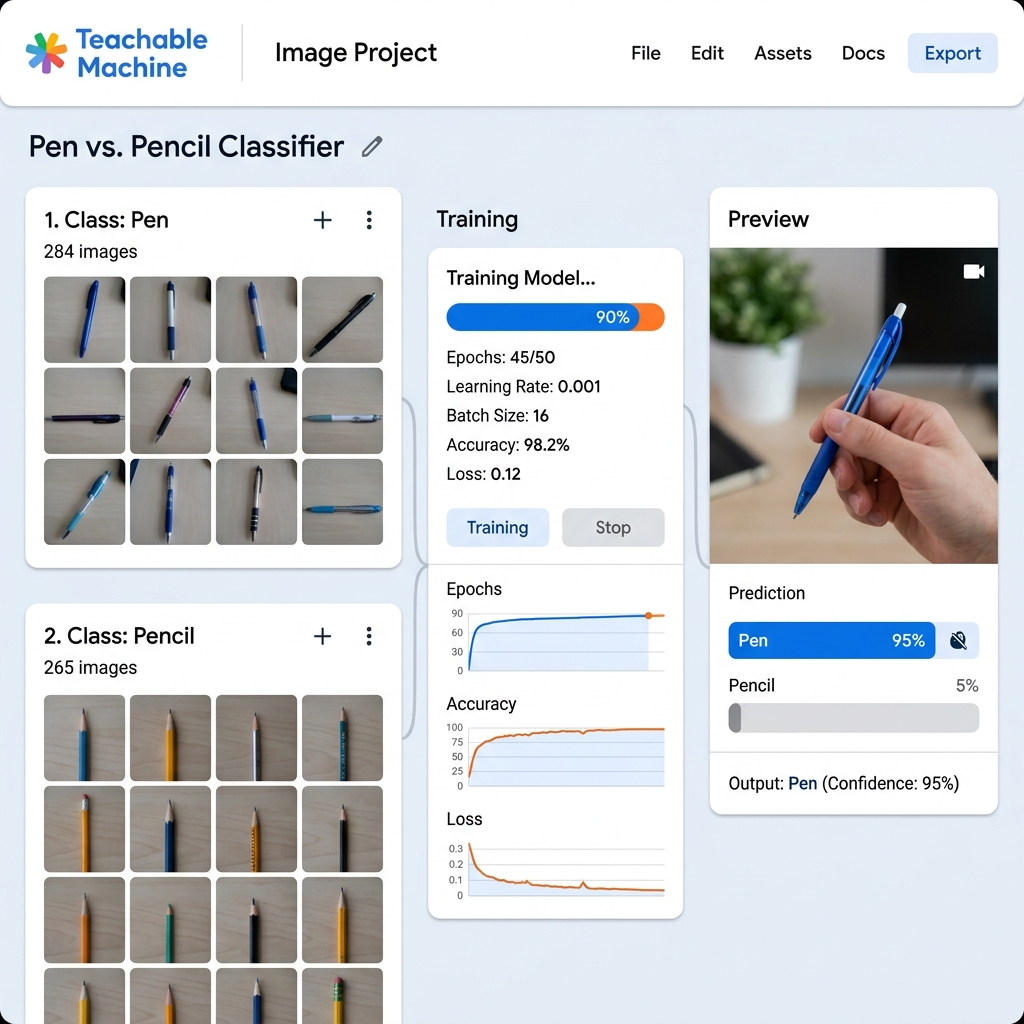
\includegraphics[width=0.82\linewidth]{images/teachable_machine_ui.jpg}
\caption[गूगल टीचेबल मशीन इंटरफ़ेस]{गूगल टीचेबल मशीन (Google Teachable Machine) का इंटरफ़ेस - जहाँ वेबकैम data द्वारा model को प्रशिक्षित किया जा रहा है।}
\label{fig:teachable-machine-ui}
\end{figure}

\section{AI के प्रकार (एक झलक)}
\begin{itemize}[leftmargin=1.4em]
  \item \eterm{Narrow AI} - केवल एक कार्य में निपुण (जैसे चेहरा पहचानना)।
        आज की लगभग सारी AI इसी प्रकार की है।
  \item \eterm{General AI} - मनुष्य जैसी सर्व-कार्य बुद्धि। यह अभी
        केवल अनुसन्धान (research) का विषय है।
\end{itemize}

\section{जनरेटिव AI एवं भाषा model (Generative AI \& LLMs)}

पिछले कुछ वर्षों में AI का एक नया रूप बहुत चर्चित हुआ है - \term{जनरेटिव
AI}{Generative AI}। यह केवल पहचानती ही नहीं, बल्कि \emph{नई सामग्री} (text, चित्र,
कोड, संगीत) स्वयं \emph{रचती} (generate) भी है। ChatGPT, Gemini एवं Claude जैसे
उपकरण इसी श्रेणी में आते हैं।

इनके मूल में \eterm{Large Language Model (LLM)} होते हैं - ऐसे
तंत्रिका जाल (neural networks) जिन्हें इंटरनेट के विशाल पाठ (text) पर प्रशिक्षित
किया जाता है। मूल रूप से ये \emph{“अगला शब्द क्या होगा”} का बार-बार पूर्वानुमान
करते हैं, और इसी से पूरे वाक्य एवं अनुच्छेद बन जाते हैं। एक सरल तंत्रिका जाल की
संरचना चित्र~\ref{fig:neural-net} में दिखाई गई है।

\begin{figure}[h]
\centering
\begin{tikzpicture}[font=\sffamily\footnotesize, >=Stealth,
    neuron/.style={circle, draw=aiblue, thick, minimum size=7mm, inner sep=0pt},
    ninp/.style={neuron, fill=ailite},
    nhid/.style={neuron, fill=aigreenL},
    nout/.style={neuron, fill=aiamberL}]
  \foreach \i in {1,2,3} \node[ninp]  (I\i) at (0, {2-\i}) {};
  \foreach \i in {1,2,3,4} \node[nhid] (H\i) at (2.2, {2.5-\i}) {};
  \foreach \i in {1,2} \node[nout] (O\i) at (4.4, {1-\i}) {};
  \foreach \i in {1,2,3} \foreach \j in {1,2,3,4} \draw[aigrey!50] (I\i) -- (H\j);
  \foreach \j in {1,2,3,4} \foreach \k in {1,2} \draw[aigrey!50] (H\j) -- (O\k);
  \node[aiblue, align=center]  at (0,1.4)   {\bfseries इनपुट\\\scriptsize Input};
  \node[aigreen, align=center] at (2.2,1.9) {\bfseries छिपी परतें\\\scriptsize Hidden};
  \node[aiamber, align=center] at (4.4,1.4) {\bfseries आउटपुट\\\scriptsize Output};
\end{tikzpicture}
\caption{एक सरल तंत्रिका जाल (neural network): इनपुट से छिपी परतों होते हुए आउटपुट तक।}
\label{fig:neural-net}
\end{figure}

\begin{jante}
ChatGPT का “GPT” का अर्थ है \emph{Generative Pre-trained Transformer}।
“Transformer” एक विशेष तंत्रिका-जाल रचना (architecture) है, जिसे सन् 2017 में
प्रस्तुत किया गया और जिसने आधुनिक भाषा मॉडलों की नींव रखी।
\end{jante}

\noindent\textbf{विज्ञान में उपयोग:} जनरेटिव AI शोध-पत्रों का सार बनाने, कोड लिखने में
सहायता, परिकल्पना (hypothesis) सुझाने, यहाँ तक कि नई औषधि-अणुओं एवं प्रोटीन-संरचनाओं
की रचना में भी सहायक है।

\begin{sochiye}
LLM कभी-कभी आत्मविश्वास से \emph{ग़लत} उत्तर भी दे देते हैं - इसे
\term{मतिभ्रम}{Hallucination} कहते हैं। इसलिए AI के उत्तर को किसी विश्वसनीय स्रोत से
सत्यापित करना क्यों आवश्यक है? कक्षा में चर्चा कीजिए।
\end{sochiye}

% ---------------- परियोजना ----------------
\begin{pariyojana}[मेरे आस-पास AI]
\textbf{उद्देश्य:} दैनिक जीवन एवं विज्ञान में AI की उपस्थिति पहचानना।\\[4pt]
\textbf{कार्य (समूह में, 3-4 विद्यार्थी):}
\begin{enumerate}[leftmargin=1.6em]
  \item एक सप्ताह तक ऐसे 10 स्थानों/उपकरणों की सूची बनाएँ जहाँ AI का उपयोग होता है
        (जैसे - मोबाइल कैमरा, YouTube सुझाव, मौसम ऐप, voice assistant)।
  \item प्रत्येक के सामने लिखें कि वह कौन-सा कार्य करती है - \emph{Perception,
        Learning, Reasoning या Decision}।
  \item इनमें से कौन-से उदाहरण किसी विज्ञान-विषय (Physics/Chemistry/Biology) से
        जुड़े हैं, चिह्नित करें।
  \item निष्कर्ष को एक पोस्टर या 5-स्लाइड प्रस्तुति (presentation) के रूप में
        कक्षा में दिखाएँ।
\end{enumerate}
\textbf{मूल्यांकन (assessment):} विविधता, वर्गीकरण की शुद्धता एवं प्रस्तुति की
स्पष्टता के आधार पर।
\end{pariyojana}

% ---------------- सारांश ----------------
\begin{bharatai}
भारत सरकार का \textbf{IndiaAI Mission} (2024) तथा \textbf{BHASHINI} परियोजना भारतीय
भाषाओं हेतु AI विकसित कर रही है - ताकि करोड़ों लोग अपनी ही भाषा में तकनीक का लाभ ले सकें।
\end{bharatai}

\section*{सारांश (Summary)}
\addcontentsline{toc}{section}{सारांश}
\begin{itemize}[leftmargin=1.4em]
  \item AI मशीनों को मानव-जैसे बौद्धिक कार्य करने योग्य बनाती है।
  \item Machine Learning, AI का वह भाग है जिसमें मशीन data से नियम स्वयं सीखती है।
  \item विशाल data के विश्लेषण में AI आधुनिक विज्ञान का शक्तिशाली उपकरण है।
  \item अंतिम वैज्ञानिक निर्णय सदैव मनुष्य के पास रहता है।
\end{itemize}

% ---------------- अभ्यास ----------------
\section*{अभ्यास (Exercises)}
\addcontentsline{toc}{section}{अभ्यास}
\textbf{अ. रिक्त स्थान भरिए:}
\begin{enumerate}[leftmargin=1.6em]
  \item \rule{2.5cm}{0.4pt}, AI का वह भाग है जिसमें मशीन data से सीखती है।
  \item आज की अधिकांश AI \rule{2.5cm}{0.4pt} (Narrow/General) प्रकार की है।
\end{enumerate}
\textbf{ब. लघु उत्तरीय:}
\begin{enumerate}[leftmargin=1.6em]
  \item परम्परागत प्रोग्रामिंग और Machine Learning में दो अंतर लिखिए।
  \item विज्ञान में AI उपयोगी होने के तीन कारण बताइए।
\end{enumerate}
\textbf{स. क्रियात्मक:}
\begin{enumerate}[leftmargin=1.6em]
  \item ऊपर की Teachable Machine गतिविधि दोहराएँ, परन्तु तीन class लेकर। accuracy
        पर क्या प्रभाव पड़ा?
\end{enumerate}

\begin{mcq}
  \item Machine Learning, निम्न में से किसका एक भाग है?
    \begin{choices}
      \item कृत्रिम बुद्धिमत्ता (AI) \item हार्डवेयर
      \item ऑपरेटिंग सिस्टम \item मॉनिटर
    \end{choices}
  \item “GPT” में अक्षर “T” किसका संक्षेप है?
    \begin{choices}
      \item Translator \item Transformer \item Transistor \item Transfer
    \end{choices}
  \item आज की अधिकांश AI किस प्रकार की है?
    \begin{choices}
      \item General AI \item Narrow AI
      \item अति-बुद्धि (Super AI) \item इनमें से कोई नहीं
    \end{choices}
  \item निम्न में से कौन-सा बुद्धिमत्ता का “Perception” कार्य है?
    \begin{choices}
      \item निष्कर्ष निकालना \item विकल्प चुनना
      \item चित्र/ध्वनि से जानकारी लेना \item नियम लागू करना
    \end{choices}
\end{mcq}

\begin{mukhyashabd}
\textbf{AI}, \textbf{Machine Learning (ML)}, \textbf{Deep Learning},
\textbf{Narrow AI}, \textbf{General AI},
\textbf{प्रत्यक्षण/अधिगम/तर्क/निर्णय}, \textbf{जनरेटिव AI (Generative AI)},
\textbf{वृहत् भाषा model (LLM)}, \textbf{Transformer}, \textbf{मतिभ्रम (Hallucination)}।
\end{mukhyashabd}
\selfcheckqr{https://kkreboot.github.io/ai-in-science-hindi/quiz/ch1.html}
